\chapter{Representation}
\label{chapter:representation}
This section develops the model used in the tracking problem. Essentially the model is two Kalman Filters which have to choose which measurement they want and end up with a bit of both.

The proposed system is based on the following two rules:
\begin{enumerate}
\item There are always two targets, both of which are described by the same motion model.
\item At every time step, save for $t=0$, each target must produce a measurement.
\end{enumerate}
This may be obvious, but it should be concretely stated. It basically ensures we don't have to introduce any new targets or discard any existing targets, which is a huge simplification.

\section{Bayes Net Representation}
\label{section:bayes_net}
\begin{figure}[!ht]
	\centering
	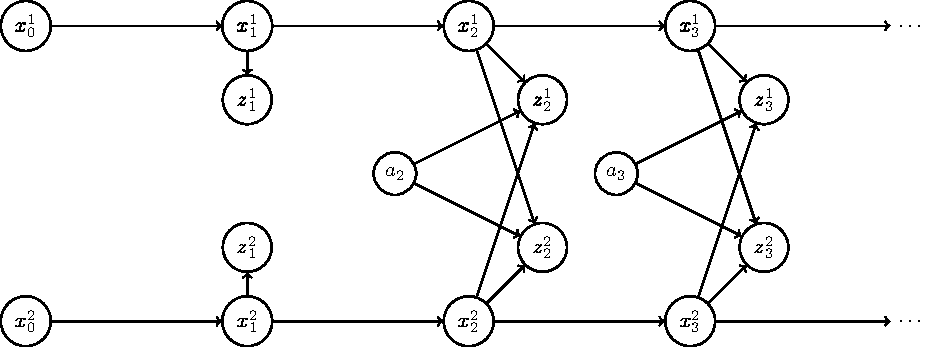
\includegraphics[scale=0.75]{tikz/bayes_net}
	\caption[A Bayes Net for a two object tracking problem.]{The initial frames for a Bayes Net modelling a two object tracking problem.}
	\label{figure:bayes_net}
\end{figure}
The Bayes Net for the system is shown in Figure~\ref{figure:bayes_net}, $a_{t}$ is the association variable while the rest is pretty much the Kalman Filter representation we've seen before. The initial belief of each state is standard Kalman filter stuff:
\begin{align}
p\left(\pmb{x}_{0}^{1}\right) &= \mathcal{N}\left( \pmb{x}_{0}^{1} | \pmb{\mu}_{0}^{1}, \Sigma_{0}^{1} \right) \\
p\left(\pmb{x}_{0}^{2}\right) &= \mathcal{N}\left( \pmb{x}_{0}^{2} | \pmb{\mu}_{0}^{2}, \Sigma_{0}^{2} \right) 
\end{align}
The prior's notation here is slightly misleading, we don't actually have specific knowledge about a target before the first measurements. All we know is that its launched on a golf course at some plausible velocity, that's hardly unique. 

The belief of the current state of an object, $\pmb{x}_{t}^{i}$, is given by the standard Kalman filter equations:
\begin{align}
p\left(\pmb{x}_{t}^{1} | \pmb{x}_{t-1}^{1} \right) &= \mathcal{N}\left( \pmb{x}_{t}^{1} | A \pmb{x}_{t-1}^{1} + B \pmb{u}, R \right) \\
p\left(\pmb{x}_{t}^{2} | \pmb{x}_{t-1}^{2} \right) &= \mathcal{N}\left( \pmb{x}_{t}^{2} | A \pmb{x}_{t-1}^{2} + B \pmb{u}, R \right)
\end{align}
The initial measurements distributions, $\pmb{z}_{1}^{1}$ and $\pmb{z}_{1}^{2}$, are standard:
\begin{align}
p\left(\pmb{z}_{1}^{1} | \pmb{x}_{1}^{1} \right) &= \mathcal{N}\left( \pmb{x}_{1}^{1} | C \pmb{x}_{1}^{1}, Q \right) \\
p\left(\pmb{z}_{1}^{2} | \pmb{x}_{1}^{2} \right) &= \mathcal{N}\left( \pmb{x}_{1}^{2} | C \pmb{x}_{1}^{2}, Q \right)
\end{align}
But measurement distributions for $t > 1$ are a bit different now:
\begin{align}
p\left(\pmb{z}_{t}^{1} | \pmb{x}_{t}^{1}, \pmb{x}_{t}^{2}, a_{t} \right) &= 
\begin{cases} 
\mathcal{N}\left( \pmb{z}_{t}^{1} | C \pmb{x}_{t}^{1}, Q \right) \mbox{if} \ a_{t} = 1 \\
\mathcal{N}\left( \pmb{z}_{t}^{1} | C \pmb{x}_{t}^{2}, Q \right) \mbox{if} \ a_{t} = 2
\end{cases} \\
p\left(\pmb{z}_{t}^{2} | \pmb{x}_{t}^{1}, \pmb{x}_{t}^{2}, a_{t} \right) &= 
\begin{cases} 
 \mathcal{N}\left( \pmb{z}_{t}^{2} | C \pmb{x}_{t}^{2}, Q \right) \mbox{if} \ a_{t} = 1 \\
\mathcal{N}\left( \pmb{z}_{t}^{2} | C \pmb{x}_{t}^{1}, Q \right) \mbox{if} \ a_{t} = 2
\end{cases}
\end{align}
The association variable, $a_{t}$:
\begin{align}
p\left(a_{t}\right) &= 
\begin{cases}
0.5 \ \mbox{if} \ a_{t} = 1 \\
0.5 \ \mbox{if} \ a_{t} = 2
\end{cases} 
\end{align}
$a_{t}$ is a binary random variable describing the probability of observation $\pmb{z}_{t}^{1}$ being caused by $\pmb{x}_{t}^{1}$  or $\pmb{x}_{t}^{2}$. If we begin with a table enumerating all four possible causal combinations and assume both objects must create distinct measurements then $a_{t} = \{ 1, 2 \}$ determines whether $\pmb{z}_{t}^{1}$ was caused by $\pmb{x}_{t}^{1}$ or $\pmb{x}_{t}^{2}$. If  $\pmb{x}_{t}^{1}$ causes a certain measurement then the remaining measurement must be caused by $\pmb{x}_{t}^{2}$.

\section{Junction Tree Representation}
\label{section:junction_tree}
\begin{figure}[!ht]
    \centering
    \begin{subfigure}[t]{0.5\textwidth}
		\centering
		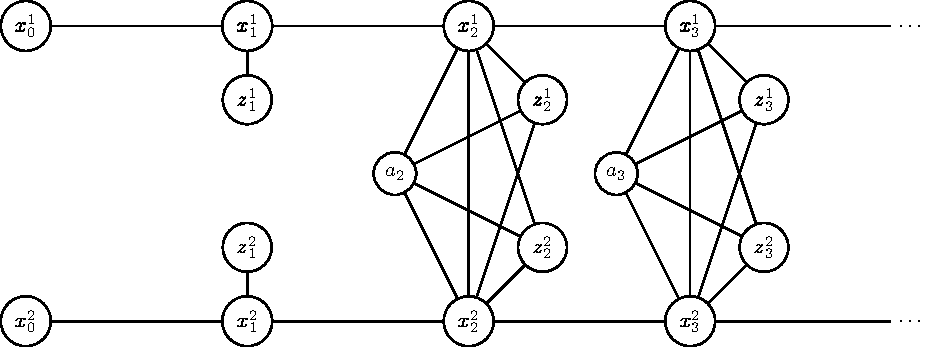
\includegraphics[height = 3cm]{tikz/moralised.pdf}
		\caption[The equivalent Markov Network.]{The moralised graph of Figure~\ref{figure:bayes_net}.}
		\label{figure:moralised}
    \end{subfigure}%   
  	~
    \centering
    \begin{subfigure}[t]{0.5\textwidth}
		\centering
		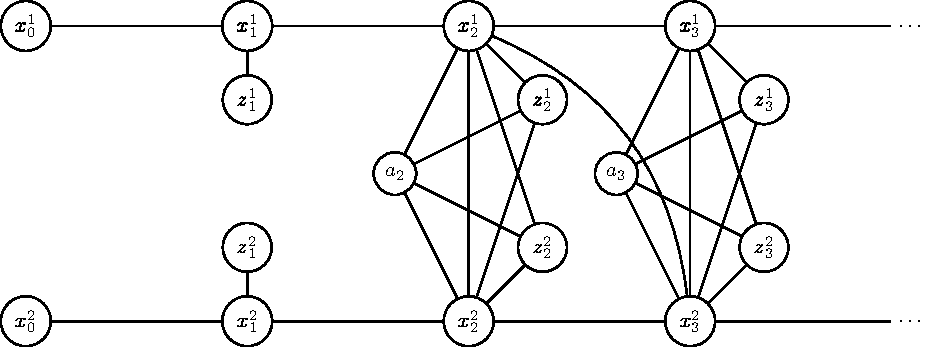
\includegraphics[height = 3cm]{tikz/induced.pdf}
		\caption[The graph induced by variable elimination.]{The graph induced by variable elimination ordering $\pmb{x}_{0}^{1}$, $\pmb{x}_{0}^{2}$, $\pmb{z}_{1}^{1}$, 			$\pmb{z}_{1}^{2}$, $\pmb{x}_{1}^{2}$, $\pmb{x}_{1}^{1}$, $\pmb{z}_{2}^{1}$, $\pmb{z}_{2}^{2}$, $a_{2}$, $\pmb{x}_{2}^{2}$, $\pmb{x}_{2}^{1}$.}
		\label{figure:induced}
    \end{subfigure}%
   	\caption{The graphs used in clique tree construction.}
    \label{figure:markov_moralised}
\end{figure}

An equivalent Junction tree will be created by applying the HUGIN algorithm to Figure~\ref{figure:bayes_net}. The undirected equivalent of the Bayes Net in Figure~\ref{figure:bayes_net} is show in Figure~\ref{figure:moralised}. After which the graph in Figure~\ref{figure:induced} is induced by variable elimination. The maximal cliques are then identified and directly used to construct Figure~\ref{figure:j_tree_1}, this graph can then be rearranged into its final, more understandable representation in Figure~\ref{figure:j_tree_2}.

The cliques in Figure~\ref{figure:j_tree_2} are assigned the following distributions:
\begin{align}
\pmb{C}_{\pmb{x} \left( 0 \right)} \left( \pmb{x}_{0}^{1},  \pmb{x}_{0}^{2} \right) &= \mathcal{N} \left( \pmb{x}_{0}^{1} | \pmb{\mu}_{0}^{1}, \Sigma_{0}^{1} \right)  \mathcal{N} \left( \pmb{x}_{0}^{2} | \pmb{\mu}_{0}^{2}, \Sigma_{0}^{2} \right) \\
\pmb{C}_{\pmb{z} \left( 1 \right)} \left( \pmb{x}_{1}^{1},  \pmb{x}_{1}^{2}, \pmb{z}_{1}^{1},  \pmb{z}_{1}^{2} \right) &=  \mathcal{N} \left( \pmb{z}_{1}^{1} | C \pmb{x}_{1}^{1}, Q \right)  \mathcal{N}   \left( \pmb{z}_{2}^{1} | C \pmb{x}_{2}^{1}, Q \right)  \\
\pmb{C}_{\pmb{x} \left( t \right)} \left( \pmb{x}_{t-1}^{1},  \pmb{x}_{t-1}^{2}, \pmb{x}_{t}^{1},  \pmb{x}_{t}^{2} \right) &=  \mathcal{N} \left( \pmb{x}_{t}^{1} | A \pmb{x}_{t-1}^{1} + B \pmb{u}, R \right)  \mathcal{N} \left( \pmb{x}_{t}^{2} | A \pmb{x}_{t-1}^{2} + B \pmb{u}, R \right)  \\
\pmb{C}_{\pmb{z} \left( t \right)} \left( \pmb{x}_{t}^{1},  \pmb{x}_{t}^{2}, \pmb{z}_{t}^{1},  \pmb{z}_{t}^{2}, a_{t} \right) &= p\left(\pmb{z}_{t}^{1} | \pmb{x}_{t}^{1}, \pmb{x}_{t}^{2}, a_{t} \right) p\left(\pmb{z}_{t}^{2} | \pmb{x}_{t}^{1}, \pmb{x}_{t}^{2}, a_{t} \right) p\left(a_{t}\right) \nonumber \\
&= \begin{cases}
 \mathcal{N}\left( \pmb{z}_{t}^{1} | C \pmb{x}_{t}^{1}, Q \right)  \mathcal{N}\left( \pmb{z}_{t}^{2} | C \pmb{x}_{t}^{2}, Q \right)  \mbox{if} \ a_{t} = 1 \\
 \mathcal{N}\left( \pmb{z}_{t}^{1} | C \pmb{x}_{t}^{2}, Q \right)  \mathcal{N}\left( \pmb{z}_{t}^{2} | C \pmb{x}_{t}^{1}, Q \right)  \mbox{if} \ a_{t} = 2 
\end{cases}
\end{align}

\begin{figure}[!ht]
	\centering
		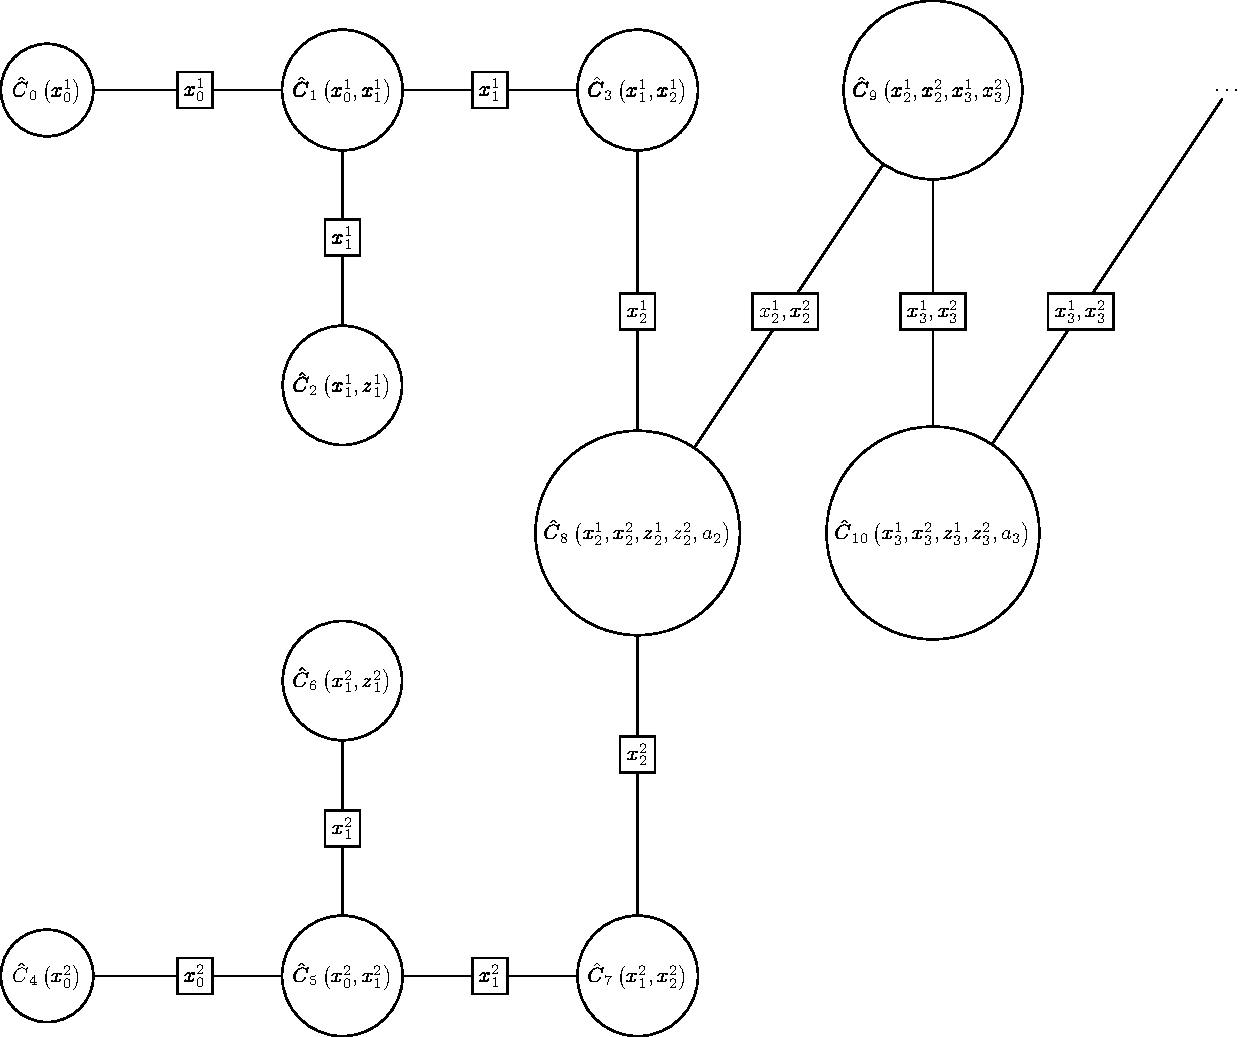
\includegraphics[scale=0.5]{tikz/j_tree_1.pdf}
		\caption[The initial Junction Tree.]{A Junction Tree constructed directly from the maximal cliques identified in Figure~\ref{figure:induced}.}
	\label{figure:j_tree_1}
\end{figure}
\begin{figure}[!ht]
	\centering
	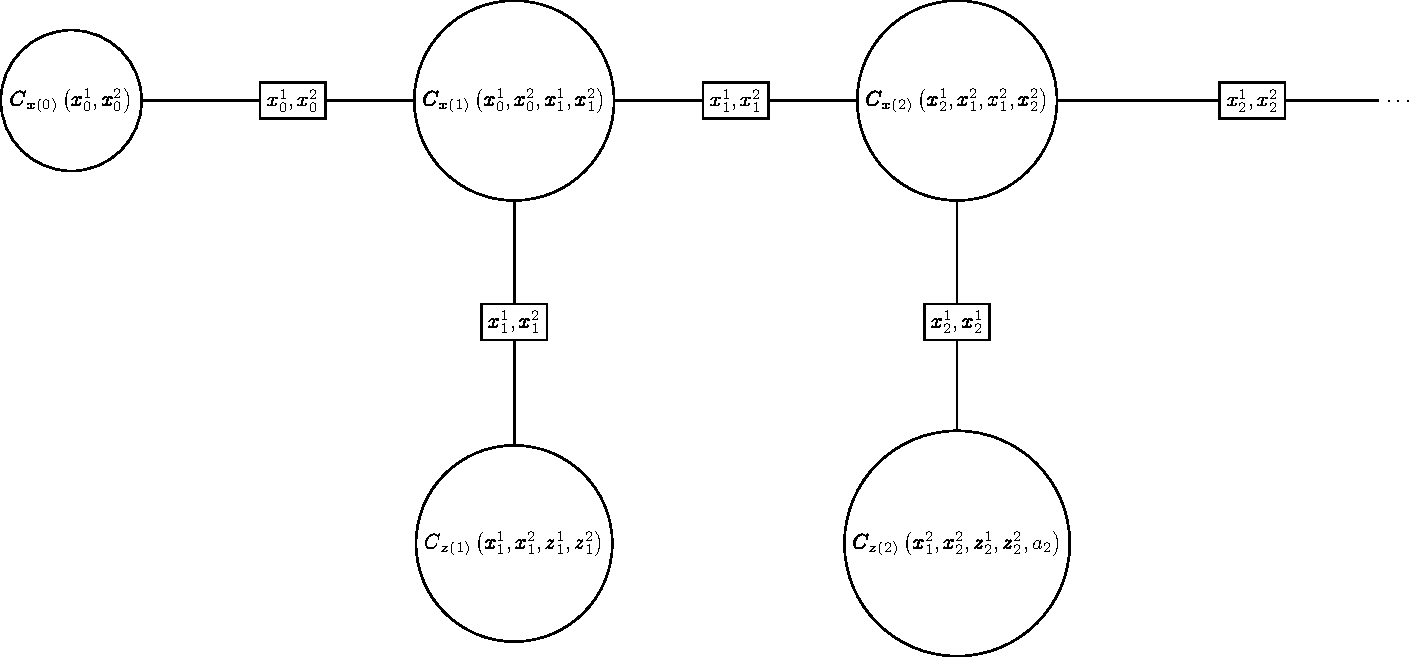
\includegraphics[scale=0.625]{tikz/j_tree_2.pdf}
	\caption[A better Junction tree.]{A better Junction Tree. This tree is equivalent to the Junction Tree in Figure~\ref{figure:j_tree_1}, but easier to analyse.}
	\label{figure:j_tree_2}
\end{figure}